\documentclass[tikz,border=0pt,11pt]{standalone}

\newcommand{\drawnuclide}[3]{%
  % Entries give the level energy, label height, and compact Nilsson label.
  \foreach \energy/\labelheight/\orbital in {#3} {
    \draw[level] (#1,\energy) -- ({#1+0.88},\energy);
    \ifnum\energy=\labelheight\relax\else
      \draw[leader] ({#1+0.88},\energy) -- ({#1+0.91},\energy)
        -- ({#1+1.00},\labelheight);
    \fi
    \node[anchor=west,inner sep=0pt,font=\footnotesize]
      at ({#1+1.05},\labelheight) {$\orbital$};
  }
  \node[anchor=north,inner sep=0pt] at ({#1+0.44},-11) {$#2$};
}

\begin{document}
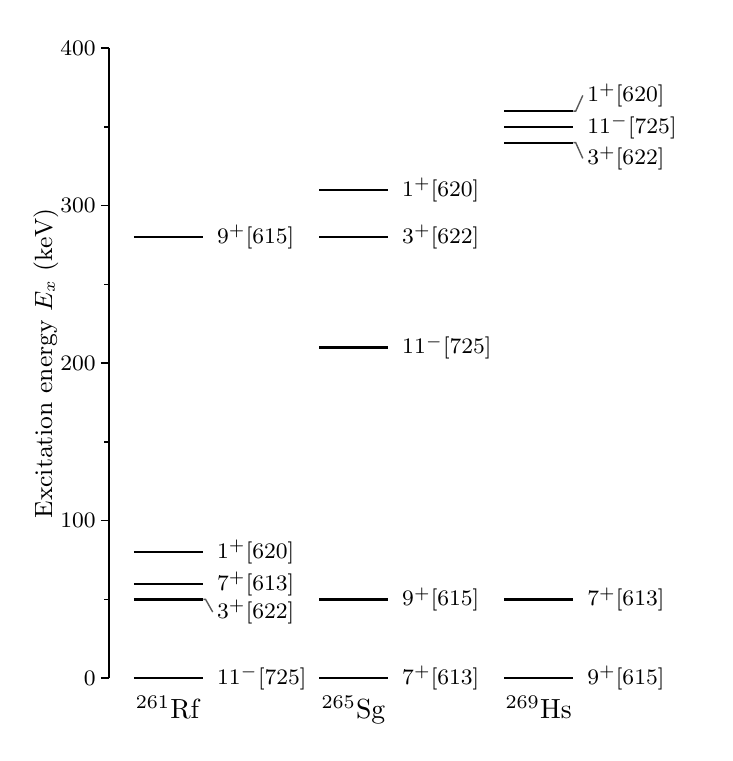
\begin{tikzpicture}[x=1cm,y=0.02cm]
  % APS single-column width. All vertical coordinates are in keV.
  \path[use as bounding box] (0,-35) rectangle (8.6,413);
  \tikzset{
    level/.style={black,line width=0.8pt},
    axis/.style={black,line width=0.55pt},
    leader/.style={black!65,line width=0.5pt}
  }

  \draw[axis] (1.03,0) -- (1.03,400);
  \foreach \energy in {0,100,200,300,400} {
    \draw[axis] (0.93,\energy) -- (1.03,\energy);
    \node[anchor=east,inner sep=0pt,font=\footnotesize]
      at (0.87,\energy) {\energy};
  }
  \foreach \energy in {50,150,250,350} {
    \draw[axis] (0.97,\energy) -- (1.03,\energy);
  }
  \node[rotate=90,inner sep=0pt,font=\small]
    at (0.23,200) {Excitation energy $E_x$ (keV)};

  % Theoretical excitation energies from nuclear_levels_tikz_codex.md.
  % Compact labels show 2 Omega instead of Omega for neutron orbitals.
  \drawnuclide{1.35}{^{261}\mathrm{Rf}}{
    0/0/11^{-}[725],50/42/3^{+}[622],60/60/7^{+}[613],
    80/80/1^{+}[620],280/280/9^{+}[615]
  }
  \drawnuclide{3.70}{^{265}\mathrm{Sg}}{
    0/0/7^{+}[613],50/50/9^{+}[615],210/210/11^{-}[725],
    280/280/3^{+}[622],310/310/1^{+}[620]
  }
  \drawnuclide{6.05}{^{269}\mathrm{Hs}}{
    0/0/9^{+}[615],50/50/7^{+}[613],340/330/3^{+}[622],
    350/350/11^{-}[725],360/370/1^{+}[620]
  }
\end{tikzpicture}
\end{document}
